\documentclass[11pt]{article}
\usepackage{amsmath}
\usepackage[hidelinks]{hyperref}
\usepackage[english]{babel}
\usepackage{graphicx}
\usepackage{wrapfig}
\usepackage{subcaption}

%Gummi|065|=)
\title{\textbf{Machine learning Nanodegree\\ Capstone project}\\ Dogs vs. Cats}

\author{Richard Deurwaarder}
\date{\today}
\begin{document}

\maketitle

\section{Problem	 Definition}

\subsection{Background}
This project is about the Kaggle competition: Dogs vs. Cats Redux: Kernels Edition\footnote{\url{https://www.kaggle.com/c/dogs-vs-cats-redux-kernels-edition}}. Originally this competition was run in 2013. In the last couple of years Machine learning has changed with techniques like Deep learning becoming more popular. For this reason Kaggle reintroduced the Dogs vs. Cats competition. Comparing the results makes for a nice view into the progression of Machine learning over the last couple of years.
\subsection{Problem statement}
The competition is about determining whether an image contains a dog or a cat. A subset of the Asirra\footnote{Animal Species Image Recognition for Restricting Access} dataset is given as part of the competition. The entire dataset has over 3 million images but for this competition we're restricted to a training set of 25,000 images, 12,500 of dogs and 12,500 images of cats. For each image our model will need to provide a probability of it containing a dog, that means give a number between 0 to 1, where 0 is definitely a cat, 1 definitely a dog.
To solve this problem I have a couple of steps to take.
\subsubsection{Analysis of the dataset}
I will need to get some information about the dataset. For instance the sizes of all the images, because I want all images to be the same size. I will also look at how the luminance varies among the images.
\subsubsection{Preprocessing of the data}
Next I will preprocess the dataset. All the image sizes need to be equal, depending on the results of the data analysis I will need to adjust the size, some might get padding, other might need to be cropped/rescaled. I will also normalize the images, making the luminance mean 0 and standard deviation 1. I might need to greyscale the images, this means every picture loses the color and instead all pixels will be in shades of gray. While this will make the images lose some information, it does reduce the amount of features by a factor 3. The intuition behind it is, lines and edges will still be there.
\subsubsection{Training the model}
Next up is actually making the predictions. I will use two different Convolutional neural networks for this task. The first one will use the Inception model\footnote{\url{https://github.com/tensorflow/models/tree/master/inception}}. This model is has the first layers pre-trained and you only train the final layer based on the categories your problem has. The intuition behind this is that the first layers identify basic elements of images: edges, corners, areas of the same color, etc. The final layer uses those basic elements to make up a category. You train that final layer for your specific problem with your specific dataset, in this case dogs and cats.\\

The second model will be a similar model to the Inception model, using convolution layers but it will be trained from scratch on our training model. I will end up choosing the best performing model.
\pagebreak[4]
\subsubsection{Evaluating the model}
To be able to choose the best performing model, I need a metric to objectively test each model. I will use two different metrics, the first is the percentage of correctly classified images. (round the probability to nearest integer). The reason for this is to be able to compare my results with the 2013 competition. For the new competition a different metric is used, I will also test each model with this metric: 

\[
LogLoss = -\dfrac{1}{n}\sum\limits^{n}_{i=1}[y_i log(\hat{y}_i) + (1-y_i)log(1-\hat{y}_i)]
\]

The main difference, between this LogLoss function and simply a percentage of correctly classified images, is this metric punishes based on how confidently wrong a model is. So when an image is of a dog, and the predictor gives a probability of 0.1 (very confident it's a cat) this metric will give a higher loss than when the predictor would've given it a 0.4 probability, even though both would be wrong.

\pagebreak[4]
\section{Analysis}
\subsection{Data Exploration}
\begin{figure}
    \centering
    \caption{Histograms of image sizes and luminances}
    \label{fig:analysis}
    \begin{subfigure}{.5\textwidth}
  	    \caption{In pixels.}
  	    \label{fig:imagesizes}
        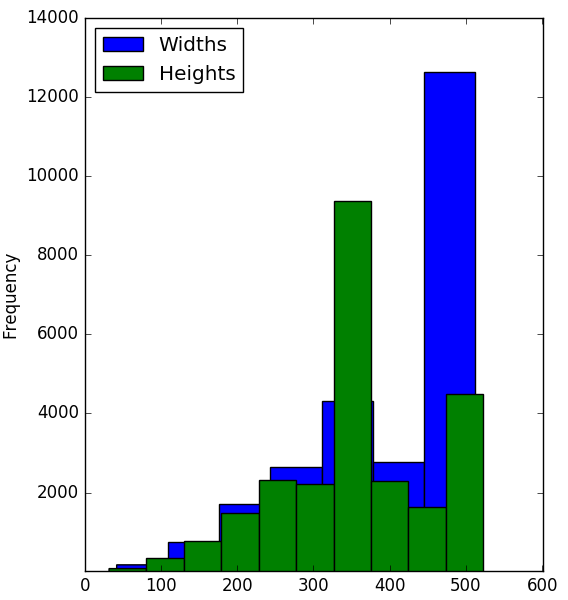
\includegraphics[width=\textwidth]{images/image_sizes}
    \end{subfigure}%
    \begin{subfigure}{.515\textwidth}
    	\caption{Mean and standard deviations.}
    	\label{fig:luminance}
    	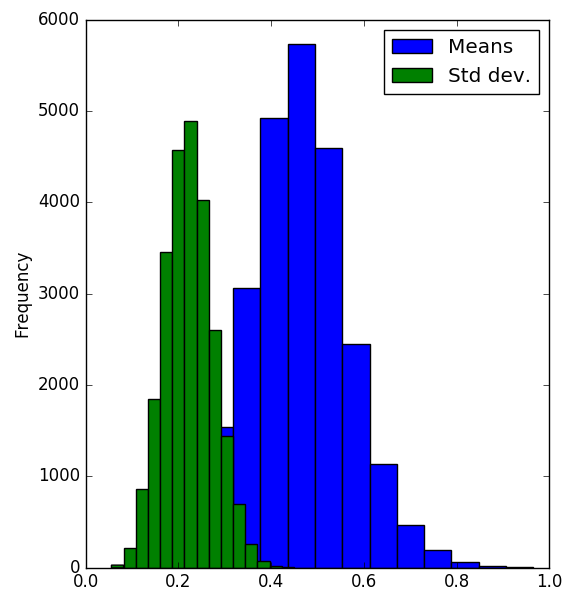
\includegraphics[width=\textwidth]{images/luminance}
    \end{subfigure}
\end{figure}
I've looked at the different sizes of the images, splitting up between widths and heights in pixels. Figure \ref{fig:imagesizes} shows a lot of images have a width of just under 500 pixels. Heights are a bit more separated, a big number has a height of around 375, and at around 500 there's another peak. What the image doesn't  show is that there are a few images (less than 10) at around 1000 pixels width and/or height.\\

Looking at the luminance of each image, the average luminance of the images is around 0.45 with the standard deviations around 0.21, see figure \ref{fig:luminance}. Normalizing could be really helpful in this case.

\begin{figure}
    \centering
    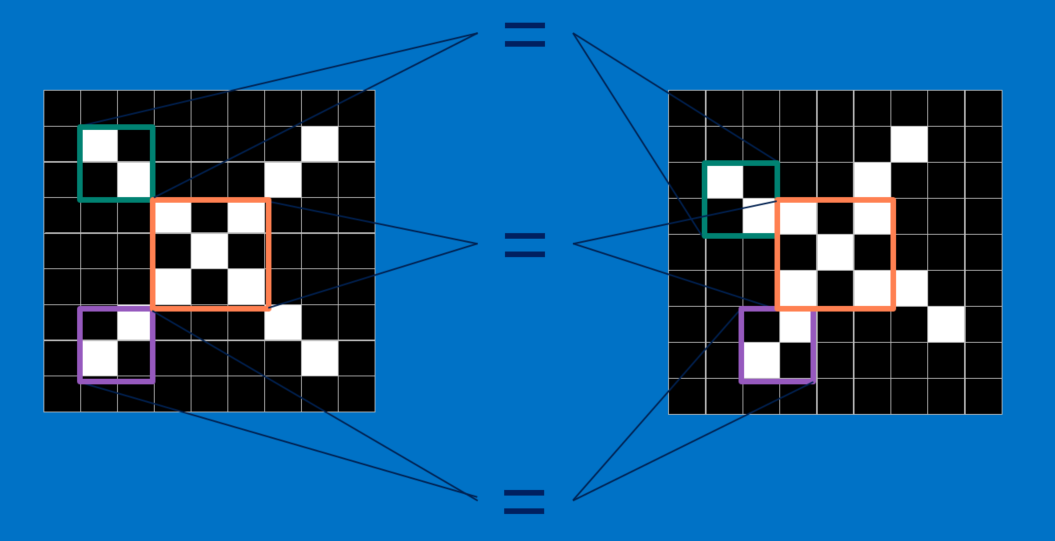
\includegraphics[width=\textwidth]{images/cnn3}
    \caption{Example of how an convolutional layer might look at an image.}
    \label{fig:cnn}
\end{figure}

\subsection{Algorithms and Techniques}
The kaggle competition specifically mentions deep learning as being one of the more promising techniques. I will be using (deep) neural networks and in particular with convolutional layers to do the image recognition.\\

Convolutional neural networks for images work by looking at a small area of the image at a time and working its way down left to right, top to bottom. For instance a convolutional layer might look at a 2 by 2, or 3 by 3 area, and look for a cross or an diagonal line. When the layers identify basic elements, it is also quite robust to rotation or translation of the objects it tries to identify. See figure \ref{fig:cnn}.\footnote{\url{https://brohrer.github.io/how_convolutional_neural_networks_work.html}}\\

The word `deep' in deep neural network comes from the fact that it has multiple layers. In this case some of those layers will be convolutional. Layers have parameters to tune. How are the weights initialized for example. Convolutional layers have even more parameters to tune, what the area will it look at (2x2, 3x3, 5x5?) What does it do with the results, max pooling, averaging? this means we have a lot of hyper-parameters to tune. 	

\subsubsection{Inception v3}
The inception model is a pre-trained model. It has been trained on a large image dataset from the ImageNet 2012 challenge, and we only have the final layer to train. This mean we don't have to tune a lot of parameters and basically have an out of the box solution.

\begin{figure}
    \centering
    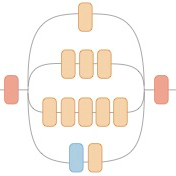
\includegraphics[width=0.25\textwidth]{images/inception-layer}
    \caption{Inception layer}
    \label{fig:inceptionlayer}
\end{figure}

\subsubsection{CNN from scratch}
For my own arcitecture I have a lot more decisions to make. But I will borrow some insights from the inception model. Have some parameters to tuneFor instance they have a specific pattern to deal with the choice on whether to take a 1x1, 3x3 or even 5x5 area. They solve this by using all of them (1x1,3x3 and 5x5) and letting the training algorithm choose. See figure \ref{fig:inceptionlayer}.


\subsection{Benchmark}
There are two sources of results. From the 2013 competition and the 2016 competition. These use different kind of metrics which cannot be converted to one or the other, so I'll compare both of them. Table \ref{leaderboard2013} shows the top 5 results and the 25th and 50th percentile of both competitions. The 2013 competition has scores ranging from 0.98 to 0.99, which will be a tough score to beat. The third column shows the 2016 scores. These scores have been accumulated from 2 September to 21 November 2016. While the competition is still ongoing, it does provide for a good baseline.

\begin{table}
\centering
\begin{tabular}{l | ll}
	\# & Score 2013 & Score 2016\\
	\hline
	1 & 0.04220 & 0.04220\\
	2 & 0.98309 & 0.04338\\
	3 & 0.98171 & 0.04557\\
	4 & 0.98171 & 0.04715\\
	5 & 0.98137 & 0.04719\\
	\hline
	25th & 0.95726 & 0.12096\\
	50th & 0.73006& 0.34584
\end{tabular}
\caption{Leaderboard for the Kaggle Dogs vs. Cats competition of 2013 and 2016. The 2013 scores are in percentage correctly classified, higher is better. The 2016 scores in LogLoss, lower is better.}
\label{leaderboard2013}
\end{table}

\section{Methodology}
\subsection{Data preprocessing}
I have chosen use a final image size of 500x500. I choose larger values rather than values which have the biggest frequency, this is because when padding an image with grey pixels (ie image that are too small and need to be bigger) I don't lose any information in the image. When having to make them smaller I need to scale them and thus lose some information which I would like to minimize.	
\subsection{Implementation}
\subsection{Refinement}
\section{Result}
\subsection{Model Evaluation and validation}
\subsection{Justification}
\section{Conclusion}
\subsection{Free-Form Visualization}
\subsection{Reflection}
\subsection{Improvement}

\end{document}
